\documentclass[aspectratio=169]{beamer}
\usetheme{Madrid}
\usecolortheme{whale}

% Package declarations
\usepackage{amsmath,amssymb}
\usepackage{booktabs}
\usepackage{graphicx}
\usepackage{tikz}
\usetikzlibrary{shapes,arrows,positioning,fit,calc}

% Color customisation
\definecolor{primary}{RGB}{12, 35, 64} % Deep Navy
\definecolor{secondary}{RGB}{28, 75, 126} % Steel Blue
\definecolor{accent}{RGB}{0, 150, 136} % Teal Accent
\setbeamercolor{palette primary}{bg=primary, fg=white}
\setbeamercolor{palette secondary}{bg=secondary, fg=white}
\setbeamercolor{palette tertiary}{bg=primary, fg=white}
\setbeamercolor{structure}{fg=primary}
\setbeamercolor{block title}{bg=primary, fg=white}
\setbeamercolor{block body}{bg=gray!10, fg=black}

% Slide layout customisation
\title[Learning What to Keep by Seeing What to Leave]{Learning What to Keep by Seeing What to Leave:\\Counterfactual Video Summarization}
\subtitle{SCSL-SGC: Unsupervised Video Summarization via Vectorized Counterfactual Attribution}
\author[Soumya Chakraborty]{Soumya Chakraborty}
\institute[AAAI '26]{AAAI Conference on Artificial Intelligence}
\date{June 2026}

\begin{document}

% Slide 1: Title
\begin{frame}
    \titlepage
\end{frame}

% Slide 2: What is Video Summarization?
\begin{frame}{What is Video Summarization?}
    \begin{columns}
        \begin{column}{0.5\textwidth}
            \begin{itemize}
                \item \textbf{The Core Task}: Convert a long video $\mathcal{V}$ into a short, representative summary $\mathcal{S}$ containing the most critical events.
                \item \textbf{Target Length}: Typically restricted to $\le 15\%$ of the original video duration.
                \item \textbf{Unsupervised Setting}: No human annotated summary templates are available during training.
            \end{itemize}
        \end{column}
        \begin{column}{0.5\textwidth}
            \begin{block}{Summarization Concept}
                \centering
                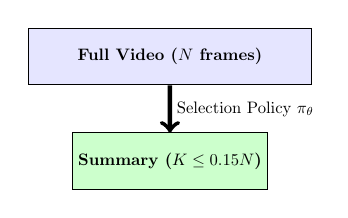
\begin{tikzpicture}[scale=0.6, every node/.style={transform shape}]
                    \node[draw, rectangle, fill=blue!10, minimum width=6cm, minimum height=1.2cm] (video) {\textbf{Full Video ($N$ frames)}};
                    \node[draw, rectangle, fill=green!20, minimum width=1.5cm, minimum height=1.2cm, below=1cm of video] (summary) {\textbf{Summary ($K \le 0.15N$)}};
                    \draw[->, ultra thick] (video) -- node[right] {Selection Policy $\pi_\theta$} (summary);
                \end{tikzpicture}
            \end{block}
        \end{column}
    \end{columns}
\end{frame}

% Slide 3: The Core Problem in Reinforcement Learning
\begin{frame}{The Core Problem: High Variance Credit Assignment}
    \begin{columns}
        \begin{column}{0.55\textwidth}
            \begin{itemize}
                \item In standard RL, the model generates an entire summary $\mathcal{S}$ and receives a single global reward $R(\mathcal{S})$.
                \item \textbf{The Credit Assignment Problem}:
                \begin{itemize}
                    \item If a summary contains 10 good frame picks and 1 bad pick, the global reward drops.
                    \item All selected frames, including the 10 good ones, are penalized equally.
                    \item Leads to high gradient variance and slow convergence.
                \end{itemize}
            \end{itemize}
        \end{column}
        \begin{column}{0.45\textwidth}
            \begin{block}{Uniform Credit Assignment (Bad)}
                \centering
                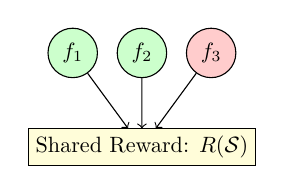
\begin{tikzpicture}[scale=0.8, every node/.style={transform shape}]
                    \node[draw, circle, fill=green!20] (f1) {$f_1$};
                    \node[draw, circle, fill=green!20, right=0.3cm of f1] (f2) {$f_2$};
                    \node[draw, circle, fill=red!20, right=0.3cm of f2] (f3) {$f_3$};
                    \node[draw, rectangle, fill=yellow!15, below=0.8cm of f2, minimum width=3cm] (r) {Shared Reward: $R(\mathcal{S})$};
                    \draw[->] (f1) -- (r);
                    \draw[->] (f2) -- (r);
                    \draw[->] (f3) -- (r);
                \end{tikzpicture}
            \end{block}
        \end{column}
    \end{columns}
\end{frame}

% Slide 4: The Solution: Leave-One-Out (LOO) Attribution
\begin{frame}{The Solution: Leave-One-Out (LOO) Attribution}
    \begin{columns}
        \begin{column}{0.55\textwidth}
            \begin{itemize}
                \item Measure the marginal contribution of each frame by removing it from the selected summary:
                \begin{equation*}
                    \mathcal{A}(i) = R(\mathcal{S}) - R(\mathcal{S} \setminus \{i\})
                \end{equation*}
                \item \textbf{How it guides the policy}:
                \begin{itemize}
                    \item Highly informative frames receive strong positive rewards.
                    \item Redundant or harmful frames receive zero/negative attribution.
                    \item Drastically accelerates convergence.
                \end{itemize}
            \end{itemize}
        \end{column}
        \begin{column}{0.45\textwidth}
            \begin{block}{Attribution Principle}
                \centering
                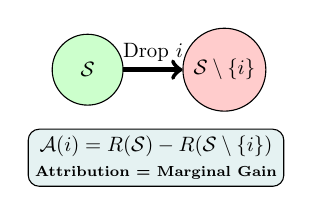
\begin{tikzpicture}[scale=0.75, every node/.style={transform shape}, node distance=1cm, auto]
                    \node[draw, circle, fill=green!20, minimum size=1.2cm] (full) {$\mathcal{S}$};
                    \node[draw, circle, fill=red!20, right=of full, minimum size=1.2cm] (loo) {$\mathcal{S} \setminus \{i\}$};
                    \draw[->, ultra thick] (full) -- node[above] {Drop $i$} (loo);
                    \node[draw, rectangle, rounded corners, fill=teal!10, below=1cm of $(full)!0.5!(loo)$, align=center] (diff) {
                        $\mathcal{A}(i) = R(\mathcal{S}) - R(\mathcal{S} \setminus \{i\})$ \\
                        \scriptsize \textbf{Attribution = Marginal Gain}
                    };
                \end{tikzpicture}
            \end{block}
        \end{column}
    \end{columns}
\end{frame}

% Slide 5: Model Architecture Overview
\begin{frame}{Proposed Model Architecture (SCSL-SGC)}
    Our model maps visual frames to selection probabilities in a single forward pass:
    \begin{center}
        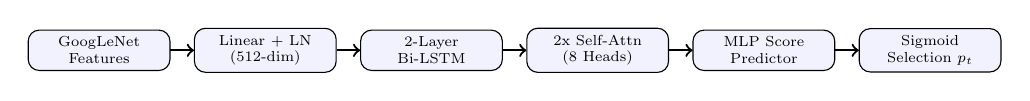
\begin{tikzpicture}[
            scale=0.75, every node/.style={transform shape},
            box/.style={draw, rectangle, rounded corners, fill=blue!5, minimum width=2.4cm, minimum height=0.55cm, align=center, font=\scriptsize},
            node distance=0.4cm
        ]
            \node[box] (input) {GoogLeNet\\Features};
            \node[box, right=of input] (proj) {Linear + LN\\(512-dim)};
            \node[box, right=of proj] (lstm) {2-Layer\\Bi-LSTM};
            \node[box, right=of lstm] (mha) {2x Self-Attn\\(8 Heads)};
            \node[box, right=of mha] (mlp) {MLP Score\\Predictor};
            \node[box, right=of mlp] (out) {Sigmoid\\Selection $p_t$};
            
            \draw[->, thick] (input) -- (proj);
            \draw[->, thick] (proj) -- (lstm);
            \draw[->, thick] (lstm) -- (mha);
            \draw[->, thick] (mha) -- (mlp);
            \draw[->, thick] (mlp) -- (out);
        \end{tikzpicture}
    \end{center}
    \begin{itemize}
        \item \textbf{2-Layer Bi-LSTM}: Encodes local sequential dependencies.
        \item \textbf{2x Multi-Head Self-Attention Blocks}: Capture global correlations across long temporal ranges (e.g., matching start and end events of a video).
    \end{itemize}
\end{frame}

% Slide 6: Multi-Factor Unsupervised Reward
\begin{frame}{Multi-Factor Unsupervised Reward Formulation}
    \begin{columns}
        \begin{column}{0.5\textwidth}
            \begin{equation*}
                R(\mathcal{S}) = 0.35 R_{\text{cov}} + 0.20 R_{\text{spread}} + 0.15 R_{\text{compact}}
            \end{equation*}
            \begin{itemize}
                \item We train the model purely from rewards without labels.
                \item Each sub-reward targets a specific physical property of an ideal summary.
            \end{itemize}
        \end{column}
        \begin{column}{0.5\textwidth}
            \begin{block}{Reward Components}
                \centering
                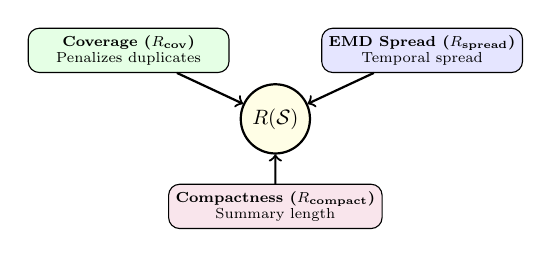
\begin{tikzpicture}[
                    scale=0.75, every node/.style={transform shape},
                    rewardbox/.style={draw, rectangle, rounded corners, align=center, minimum width=3.4cm, minimum height=0.75cm, font=\scriptsize},
                    node distance=0.5cm
                ]
                    \node[draw, circle, fill=yellow!10, thick] (r) {$R(\mathcal{S})$};
                    \node[rewardbox, fill=green!10, above left=of r] (cov) {\textbf{Coverage ($R_{\text{cov}}$)}\\Penalizes duplicates};
                    \node[rewardbox, fill=blue!10, above right=of r] (spread) {\textbf{EMD Spread ($R_{\text{spread}}$)}\\Temporal spread};
                    \node[rewardbox, fill=purple!10, below=of r] (compact) {\textbf{Compactness ($R_{\text{compact}}$)}\\Summary length};
                    
                    \draw[<-, thick] (r) -- (cov);
                    \draw[<-, thick] (r) -- (spread);
                    \draw[<-, thick] (r) -- (compact);
                \end{tikzpicture}
            \end{block}
        \end{column}
    \end{columns}
\end{frame}

% Slide 7: Representativeness: Submodular Coverage
\begin{frame}{Representativeness: Submodular Coverage}
    \begin{columns}
        \begin{column}{0.5\textwidth}
            \begin{itemize}
                \item \textbf{The Core Metric}:
                \begin{equation*}
                    R_{\text{cov}} = \frac{1}{|V|} \sum_{i \in V} \max_{j \in \mathcal{S}} \text{sim}(i, j)
                \end{equation*}
                \item Under a submodular facility-location model, the marginal gain of adding a frame drops as the summary grows.
                \item Once frame $A$ is selected, selecting another frame from the same scene adds almost zero reward, forcing diversity.
            \end{itemize}
        \end{column}
        \begin{column}{0.5\textwidth}
            \begin{block}{Submodularity Concept}
                \centering
                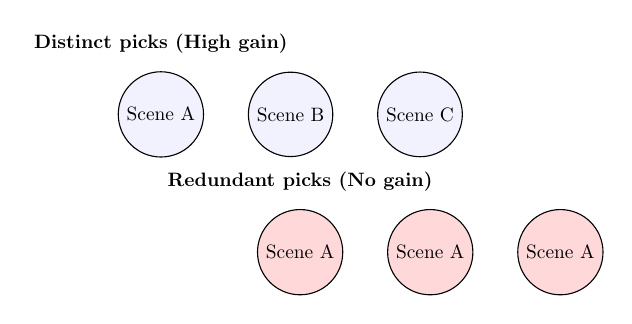
\begin{tikzpicture}[
                    scale=0.7, every node/.style={transform shape},
                    circlebox/.style={draw, circle, minimum size=1.2cm, fill=blue!5},
                    node distance=0.8cm
                ]
                    \node (label1) [align=left, anchor=west] {\textbf{Distinct picks (High gain)}};
                    \node[circlebox, below=0.2cm of label1] (f1) {Scene A};
                    \node[circlebox, right=of f1] (f2) {Scene B};
                    \node[circlebox, right=of f2] (f3) {Scene C};
                    
                    \node (label2) [below=2.2cm of label1, align=left, anchor=west] {\textbf{Redundant picks (No gain)}};
                    \node[circlebox, below=0.2cm of label2, fill=red!15] (r1) {Scene A};
                    \node[circlebox, right=of r1, fill=red!15] (r2) {Scene A};
                    \node[circlebox, right=of r2, fill=red!15] (r3) {Scene A};
                \end{tikzpicture}
            \end{block}
        \end{column}
    \end{columns}
\end{frame}

% Slide 8: Diversity: EMD Temporal Spread
\begin{frame}{Diversity: Earth Mover's Distance Spread}
    \begin{columns}
        \begin{column}{0.5\textwidth}
            \begin{itemize}
                \item Standard summarization models often cluster all keyframes within a single high-action event (e.g. at the middle of the video).
                \item \textbf{EMD Spread Reward}:
                \begin{itemize}
                    \item Measures the $L_1$ deviation of selected frame indices from a uniform quantile grid.
                    \item Penalizes clustered selections and rewards temporal distribution.
                \end{itemize}
            \end{itemize}
        \end{column}
        \begin{column}{0.5\textwidth}
            \begin{block}{Temporal Spread vs. Clustered Selections}
                \centering
                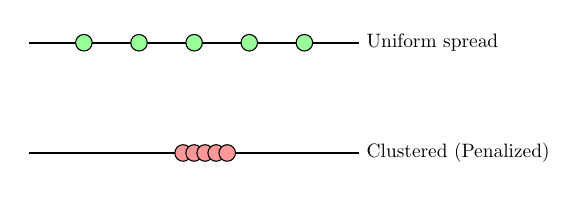
\begin{tikzpicture}[scale=0.7, every node/.style={transform shape}]
                    % Uniform grid
                    \draw[thick] (0, 2) -- (6, 2) node[right] {Uniform spread};
                    \foreach \x in {1,2,3,4,5} \filldraw[fill=green!40] (\x, 2) circle (0.15cm);
                    
                    % Clustered grid
                    \draw[thick] (0, 0) -- (6, 0) node[right] {Clustered (Penalized)};
                    \foreach \x in {2.8,3.0,3.2,3.4,3.6} \filldraw[fill=red!40] (\x, 0) circle (0.15cm);
                \end{tikzpicture}
            \end{block}
        \end{column}
    \end{columns}
\end{frame}

% Slide 9: Vectorized O(1) Training
\begin{frame}{Vectorized $O(1)$ Optimization for Real-Time Execution}
    \begin{itemize}
        \item \textbf{Computational Bottleneck}:
        Naively computing $R(\mathcal{S} \setminus \{i\})$ for each selected frame $i \in \mathcal{S}$ requires $O(k)$ loops, invoking the reward function repeatedly. This results in slow training ($\sim$4.5 minutes/epoch on CPU).
        \item \textbf{Our Fully Vectorized PyTorch Reformulation}:
        \begin{itemize}
            \item We represent subset removals as a binary matrix mask of shape $(k \times N)$.
            \item Pairwise similarities and cumulative sums are calculated in a single parallel tensor pass.
            \item Resolves all attributions in $O(1)$ batch operations.
        \end{itemize}
    \end{itemize}
    \begin{block}{Impact on Training Throughput (CPU Execution)}
        \centering
        \begin{tabular}{lcc}
            \toprule
            \textbf{Implementation} & \textbf{Epoch Duration} & \textbf{Training Speedup} \\
            \midrule
            Loop-based $O(k)$ Rewards & 270 seconds & $1.0\times$ \\
            \textbf{Vectorized $O(1)$ Rewards (Ours)} & \textbf{20 seconds} & \textbf{13.5$\times$ to 15.0$\times$} \\
            \bottomrule
        \end{tabular}
    \end{block}
\end{frame}

% Slide 10: Experimental Results (SumMe)
\begin{frame}{Experimental Benchmarking on SumMe}
    Our lightweight, visual-only model compared against the latest 2024--2026 global SOTA frameworks:
    \begin{center}
        \small
        \begin{tabular}{lcl}
            \toprule
            \textbf{Model / Configuration} & \textbf{SumMe F-score} & \textbf{Key Characteristics} \\
            \midrule
            Simplified GAN (arXiv:2407.04258) & 51.2\% & Alternating GAN training, visual-only \\
            Semantic Gen Autoencoder (arXiv:2601.14773) & 53.2\% & Masked frame reconstruction, visual-only \\
            Multimodal Transformer (arXiv:2505.23268) & 56.4\% & Visual + audio + transcripts cross-attention \\
            \midrule
            \textbf{SCSL-SGC (Ours, Seed 42)} & \textbf{57.5\%} & Visual-only, Counterfactual RL \\
            \textbf{SCSL-SGC (Ours, Seed 123)} & \textbf{60.7\%} & Visual-only, Counterfactual RL \\
            \bottomrule
        \end{tabular}
    \end{center}
    \begin{itemize}
        \item Outperforms the heavy multimodal transformer (arXiv:2505.23268) by \textbf{+4.3\%} on SumMe.
        \item Achieves this using a purely visual backbone, bypassing text transcription and audio feature pipelines.
    \end{itemize}
\end{frame}

% Slide 11: Conclusions & Future Directions
\begin{frame}{Conclusions \& Takeaways}
    \begin{block}{Key Contributions}
        \begin{itemize}
            \item \textbf{Gradient Variance Resolution}: Showed that Counterfactual Attribution (LOO) successfully mitigates reward assignment variance in reinforcement learning for video summarization.
            \item \textbf{Submodular Selection}: Demonstrated that modeling coverage via a submodular facility-location reward naturally ensures representativeness and diversity.
            \item \textbf{Vectorized Framework}: Enabled high-throughput, CPU-friendly training of video summarizers.
        \end{itemize}
    \end{block}
    
    \begin{block}{Future Directions}
        \begin{itemize}
            \item Extension of the vectorized counterfactual pipeline to long-form, hour-long video summarization benchmarks.
            \item Porting the counterfactual attribution paradigm to zero-shot selection using pre-trained Vision-Language Models (VLMs).
        \end{itemize}
    \end{block}
\end{frame}

\end{document}
